\subsection{Age and time of interaction}

In opposition to the previous section we now focus on the temporal variable of $P_\text{nst}$ which is the age of interaction. 
We provide quantitative representations of the interaction duration using the age distribution,
\begin{equation*}
    P_a(\textbf{x},t,a)
    = \int_{\mathbb{R}^3}
    P_\text{nst}(\textbf{x},\textbf{r},t,a)
    d\textbf{r}. 
\end{equation*} 
From this definition we can also define a major temporal quantity, which is the destruction rate, $1/\tau_a$ or the mean age, defined as,  
\begin{equation}
    \tau_a(\textbf{x},t)
    = \int_{\mathbb{R}^3}
     \int_{0}^\infty
    a P_\text{nst}(\textbf{x},\textbf{r},t,a)
    d\textbf{r}. 
    da, 
    \label{eq:mean_time}
\end{equation} 
It is also possible to derive an analytical formula for the age distribution under the \textit{random destruction assumption}\citep{zhang2023evolution}.
In other worlds,  we consider that the probability of particle pair destruction is uncorrelated with the age of interaction, or that any pairs of nearest neighbor can be broken apart equally likely regardless of the current age of the particle pair. 
Let us define $1/\tau_a$ as the rate of pair destruction, then this hypothesis state that $\tau_a$ is not a function of the age.  
Under this assumption, we can derive an analytical formula for the age distribution \citep{zhang2023evolution}, 
\begin{align}
    P_a(\textbf{x},t, a)  
    =\frac{e^{-a/\avgcond{\tau_d}(\textbf{x},t)}}{\avgcond{\tau_d}(\textbf{x},t)},
    \label{eq:Pa}
\end{align} 
Therefore, under this assumption the time measure of the micro scale interaction can be entirely described by the mean age $\tau_a$. 

In \ref{fig:age_picture} (left) we display the dimensionless age distribution $P_a(a)$ for $\phi = 0.01,0.05,0.1,0.2$. 
Note that the age is made dimensionless using the inertial time scale, $\sqrt{g/d_p^3}$ where $d_p$ is the length scale between two particles defined as $d_p = n_p^{-3}(\textbf{x},t)$. 
It is seen that for most of the case the distribution are rather well represented by the distribution from \ref{eq:Pa}, implying that the random destruction assumption holds true for most of the cases. 
\begin{figure}[h!]
    \centering
    % 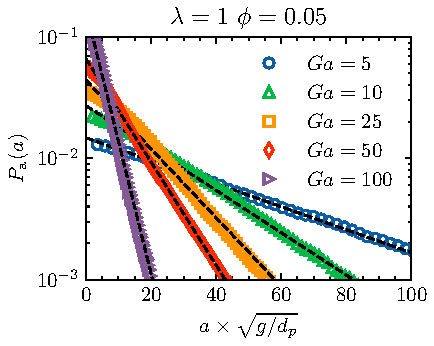
\includegraphics[height = 0.3\textwidth]{image/HOMOGENEOUS_NEW/Dist/Pa_l_1_PHI_5.pdf}
    % 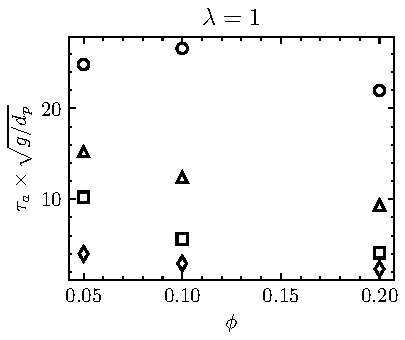
\includegraphics[height = 0.3\textwidth]{image/HOMOGENEOUS_NEW/tau_PHI_l_1.pdf}

    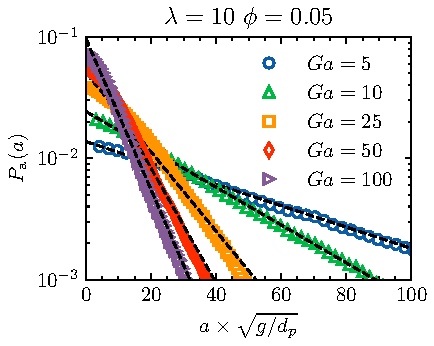
\includegraphics[height = 0.3\textwidth]{image/HOMOGENEOUS_NEW/Dist/Pa_l_10_PHI_5.pdf}
    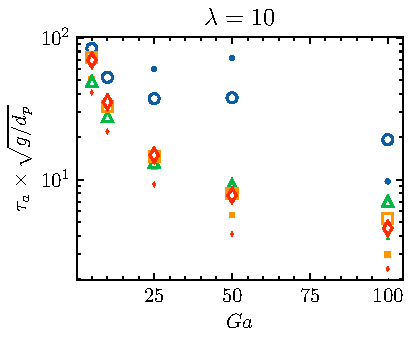
\includegraphics[height = 0.3\textwidth]{image/HOMOGENEOUS_NEW/tau_PHI.pdf}
    \caption{(left) Age distribution function $P_a(a)$ in terms of the dimensionless age : $a \sqrt{g/d_p}$, for $\lambda = 1$ and  $\phi = 0.05$.
    (dashed lines) Theoretical age distribution, see \ref{eq:Pa}. 
    (right) Mean dimensionless age $\tau_a =  \int_0^\infty aP_a(a)da$ in terms of the volume fraction $\phi$.  
    ($\bigcirc$) $Ga=10$; ($\triangle$) $ Ga = 25$; ($\square$) $Ga = 50$ ($\lozenge$) $Ga =100$.
    The white symbols correspond to $\lambda = 1$, and black symbols to $\lambda = 10$. }
    \label{fig:age_picture}
\end{figure}
Nevertheless, we can remark that for $\lambda = 10$, $\phi = 0.05,0.1$ the distribution slightly differ from a strait line. 
In fact, it is seen that the age distribution reconstructed with DNS for these parameters exhibit a higher density for low ages and less for higher age compared to the random distribution.
Apart from these two case it is reasonable to say that \ref{eq:Pa} is well representative of the age distribution. 
Regarding the low inertial regime, in 
\begin{enumerate}
    \item The random assumption works well except for the low volume fraciton displayed in appendix
    \item The time of interaction decrease with high $Ga$ and $\lambda = 10$.
    \item And clearly is non-monotonic with the volume fraction even if it seems to decrease. 
\end{enumerate}


For a better understanding of the age meaning, in the expression of $\textbf{w}^\text{nst}(\textbf{r},a)$ we first study a simpler probability density. 
Indeed, we restrict our attention to the age-conditioned relative normal velocity fields, 
\begin{equation*}
    w^\text{nst-r}_n(a)P_\text{nst-r}(a)
    = \int_{\mathbb{R}^3}
    \textbf{n} \cdot \textbf{w}^\text{nst}
    P_\text{nst}(\textbf{r},a) d\textbf{r}
\end{equation*}
where \textbf{n} is the unit vector define by $\textbf{n} = \textbf{r}/ |\textbf{r}|$. 
In this way $w^\text{nst-r}_n(a)$ is the average relative normal velocity between the nearest pair of particles at age $a$. 
Therefore, it describes the approach velocity from one particle to another in average along the interaction time. 
\begin{figure}[h!]
    \centering
    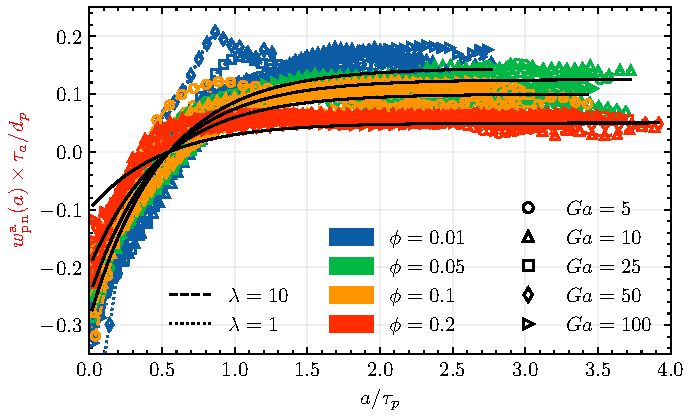
\includegraphics[height = 0.8\textwidth]{image/HOMOGENEOUS_NEW/Age_cond/uR_rel.pdf}
    % \includegraphics[height = 0.3\textwidth]{image/HOMOGENEOUS_NEW/Age_cond/r_l_10_PHI_10.pdf}
    \caption{(left) Relative normal approach velocity between two nearest neighbors, averaged conditionally on the age of interaction.  
    The age, $a/\tau_a$ as well as the velocity are made dimensionless  with the mean age $\tau_a$ and the length scale $d_p = n_p^{-1/3}$. 
    The symbols represent the different \textit{Galileo} numbers,
    ($\bigcirc$) $Ga=10$; ($\triangle$) $ Ga = 25$; ($\square$) $Ga = 50$ ($\lozenge$) $Ga =100$.
    The colors represent the different volume fractions, (blue) $\phi =0.01$, (green) $\phi = 0.05$ (organ) $\phi=0.1$ (red) $\phi = 0.2$. 
    The white symbols correspond to $\lambda = 1$, and black symbols to $\lambda = 10$. 
    (colored dashed lines) $\lambda = 1$. 
    (black dashed lines) $a/\tau_a =1$. 
    We observe that all velocity scales with $d_p$ and $\tau_a$. 
    }
    \label{fig:normal_vel_picture}
\end{figure}

\begin{itemize}
    \item Major conclusion of this part is that $\tau_a$ and $d_p$ are the time and length scale driving the relative kinematic between particles. 
    \item $\tau_d$ varies non-monotonically between the cases. 
    \item the age dist i random
\end{itemize}